\chapter{Algorithms}

\selectlanguage{english}

\section{Reject Inference methods} \label{app1:reject}

\subsection{Fuzzy Augmentation} \label{fuzzy}

Fuzzy Augmentation can be found in \cite{economix}; it is the following procedure:
\begin{enumerate}
\item Construct Scorecard "Known Good Bad" (KGB) $S^{\text{f}}$ with financed clients' data (Figure \ref{fuzzy:sfig1})
\item Calculate $p(1|x,\hat{\theta}^{\text{f}}) = \text{logit}(S^{\text{f}}(x))$ for rejects (Figure \ref{fuzzy:sfig2})
\item Infer rejected client $i$ as good with weight $p(1|x,\hat{\theta}^{\text{f}})$ and as bad with weight {\begin{sloppypar} $1-p(1|x,\hat{\theta}^{\text{f}})$ (Figures \ref{fuzzy:sfig2} and \ref{fuzzy:sfig3}) \end{sloppypar} }
\item Calibrate a new scorecard with the ‘‘augmented'' dataset (Figure \ref{fuzzy:sfig4})
\end{enumerate}

\begin{table}
\caption{\label{fuzzyexample} Example of implementation of the Fuzzy Augmentation method on a small dataset}
{\setlength{\parindent}{0cm}
\begin{multicols}{4}
\small

\begin{subfigure}[t]{0.22\textwidth}
\begin{center}
\begin{adjustbox}{max width=0.95\textwidth}
\begin{tabular}{l l}
\toprule
\textbf{${\bm{y}}^{\text{f}}$} & \textbf{${\bm{x}}^{\text{f}}$}\\
\midrule
1 & 0.562 \\
1 & 0.910 \\
0 & 0.430 \\
\bottomrule
\end{tabular}
\end{adjustbox}
\end{center}

\subcaption{Scorecard $S^{\text{f}}$ on financed loans}
\label{fuzzy:sfig1}
\end{subfigure}

\columnbreak

\begin{subfigure}[t]{0.22\textwidth}
\begin{center}
\begin{adjustbox}{max width=0.95\textwidth}
\begin{tabular}{l l l}
\toprule
\textbf{Weight} & \textbf{$\hat{\bm{y}}^{\text{nf}}$} & \textbf{${\bm{x}}^{\text{nf}}$}\\
\midrule
0.68 & 1 & 0.347 \\
0.10 & 1 & 0.140 \\
0.35 & 1 & 0.295 \\
\bottomrule
\end{tabular}
\end{adjustbox}
\end{center}

\caption{Inferred good not financed loans and their weights}
\label{fuzzy:sfig2}
\end{subfigure}

\columnbreak

\begin{subfigure}[t]{0.22\textwidth}
\begin{center}
\begin{adjustbox}{max width=0.95\textwidth}
\begin{tabular}{l l l}
\toprule
\textbf{Weight} & \textbf{$\hat{\bm{y}}^{\text{nf}}$} & \textbf{${\bm{x}}^{\text{nf}}$}\\
\midrule
0.32 & 0 & 0.347 \\
0.90 & 0 & 0.140 \\
0.65 & 0 & 0.295 \\
\bottomrule
\end{tabular}
\end{adjustbox}
\end{center}

\caption{Inferred bad not financed loans and their weights}
\label{fuzzy:sfig3}
\end{subfigure}

\columnbreak

\begin{subfigure}[t]{0.22\textwidth}
\begin{center}
\begin{adjustbox}{max width=0.95\textwidth}
\begin{tabular}{l l l}
\toprule
\textbf{Weight} & \textbf{${\bm{y}}$} & \textbf{${\bm{x}}$}\\
\midrule
1 & 0 & 0.562 \\
1 & 1 & 0.910 \\
1 & 0 & 0.430 \\
0.68 & 1 & 0.347 \\
0.10 & 1 & 0.140 \\
0.35 & 1 & 0.295 \\
0.32 & 0 & 0.347 \\
0.90 & 0 & 0.140 \\
0.65 & 0 & 0.295 \\
\bottomrule
\end{tabular}
\end{adjustbox}
\end{center}
\caption{Fuzzy augmented learning dataset}
\label{fuzzy:sfig4}
\end{subfigure}

\end{multicols}
}
\end{table}

 Clearly:

 \[ \forall j = 1, \ldots, d, \: \frac{\partial \sum_{i=n+1}^{m+n} \sum_{y_i = 0}^{1} p(y_i^{\text{inf}}| x_i, \hat{\theta}^{\text{f}})\ln (p(y_i| x_i, \theta))}{\partial \theta_j} = 0 \Leftrightarrow \theta = \hat{\theta}^{\text{f}} \]

 It can be shown that:
 \[\argmax_{\theta \in \Theta}  \sum_{i=n+1}^{m+n} \sum_{y_i = 0}^{1} p_{\hat{\theta}^{\text{f}}}(y_i| x_i)\ln (p_\theta(y_i| x_i)) = \hat{\theta}^{\text{f}}\]

 And finally:
 \[\argmax_{\theta \in \Theta} \ell(\theta;{\bm{x}},{\bm{y}}^{\text{f}},{\bm{y}}^{\text{inf}}) = \argmax_{\theta \in \Theta} \ell(\theta;{\bm{x}},{\bm{y}}^{\text{f}}) = \hat{\theta}^{\text{f}}\]

 To conclude, this method will not change the estimated parameters of any discriminant model, asymptotically and with a finite set of observations, regardless of any assumption on the missingness mechanism or the true model hypothesis. In other words, Fuzzy Augmentation has no effect on the Kullback-Leibler divergence, making this method useless because it is no different than the accepted clients model minimizing asymptotically expression~$H^{\text{f}}_{\theta}$ and not expression~$H_{\theta}$.


\subsection{Reclassification} \label{reclassification}

Reclassification can be found in \cite{RI6}, also sometimes referred to as extrapolation as in \cite{banasik}; it is the following procedure:
\begin{enumerate}
\item Construct Scorecard "Known Good Bad" (KGB) $S^{\text{f}}$ with financed clients' data (Figure~\ref{reclass:sfig1})
\item Calculate $p(1|x,\hat{\theta}^{\text{f}}) = \text{logit}(S^{\text{f}}(x))$ for rejects
\item Infer default status of rejected client $i$ if $S^{\text{f}}(x) > \text{threshold}$; typically threshold $=0.5$ (Figure~\ref{reclass:sfig2})
\item Calibrate a new scorecard with the ‘‘augmented'' dataset (Figure~\ref{reclass:sfig3})
\end{enumerate}

\begin{table}
\caption{\label{reclassexample} Example of implementation of the Reclassification method on a small dataset}
{\setlength{\parindent}{0cm}
\begin{multicols}{3}

\begin{subfigure}[t]{0.31\textwidth}
\begin{center}
\begin{adjustbox}{max width=\textwidth}
\begin{tabular}{l l}
\toprule
\textbf{${\bm{y}}^{\text{f}}$} & \textbf{${\bm{x}}^{\text{f}}$}\\
\midrule
1 & 0.562 \\
1 & 0.910 \\
0 & 0.430 \\
\bottomrule
\end{tabular}
\end{adjustbox}
\end{center}

\caption{Development of scorecard $S^{\text{f}}$ on financed clients}
\label{reclass:sfig1}
\end{subfigure}


\columnbreak

\begin{subfigure}[t]{0.31\textwidth}
\begin{center}
\begin{adjustbox}{max width=\textwidth}
\begin{tabular}{l l l}
\toprule
\textbf{$p(1|x,\hat{\theta}^{\text{f}})$} & \textbf{$\hat{\bm{y}}^{\text{nf}}$} & \textbf{${\bm{x}}^{\text{nf}}$}\\
\midrule
0.68 & 1 & 0.347 \\
0.10 & 0 & 0.140 \\
0.35 & 0 & 0.295 \\
\bottomrule
\end{tabular}
\end{adjustbox}
\end{center}

\caption{We force $y^{\text{nf}}=1$ if $\text{logit}(S^{\text{f}}(x)) \geq 0.5$}
\label{reclass:sfig2}
\end{subfigure}

\columnbreak

\begin{subfigure}[t]{0.31\textwidth}
\begin{center}
\begin{adjustbox}{max width=\textwidth}
\begin{tabular}{l l}
\toprule
\textbf{${\bm{y}}$} & \textbf{${\bm{x}}$}\\
\midrule
0 & 0.562 \\
1 & 0.910 \\
0 & 0.430 \\
1 & 0.347 \\
0 & 0.140 \\
0 & 0.295 \\
\bottomrule
\end{tabular}
\end{adjustbox}
\end{center}
\caption{Reclassified learning dataset}
\label{reclass:sfig3}
\end{subfigure}

\end{multicols}
}
\end{table}


\subsection{Augmentation} \label{augmentation}

\begin{enumerate}
\item Construct Scorecard "Accept Reject" (ACRJ) $R$ with financed clients' data on target variable $Z$ (Figure~\ref{augment:sfig1})
\item Create $K$ score bands $B_1, \ldots, B_K$ according to $R$
\item Compute in each score band $\hat{p}_{\text{true}}(\text{f}|x \in B_k) = \dfrac{|B_k|}{|z=\text{f}|}$ (Figure~\ref{augment:sfig2})
\item Construct Scorecard $S$ on target variable Good/Bad with financed clients' data re-weighted (Figure~\ref{augment:sfig3})
\end{enumerate}

\begin{table}
\caption{\label{augmentexample} Example of implementation of the Augmentation method on a small dataset}
{\setlength{\parindent}{0cm}
\begin{multicols}{3}

\begin{subfigure}[t]{0.31\textwidth}
\begin{center}
\begin{adjustbox}{max width=0.95\textwidth}

\begin{tabular}{l l l}
\toprule
\textbf{${\bm{y}}$} & \textbf{${\bf{z}}$} & \textbf{Score-band}\\
\midrule
1 & \text{f} & 1 \\
1 & \text{f} & 1 \\
0 & \text{f} & 1 \\
NA & \text{nf} & 1 \\
NA & \text{nf} & 1 \\
NA & \text{nf} & 1 \\
... & ... & ... \\
\bottomrule
\end{tabular}
\end{adjustbox}
\end{center}

\caption{Calculation of $K$ score-bands on the ACRJ score}
\label{augment:sfig1}
\end{subfigure}

\columnbreak

\begin{subfigure}[t]{0.31\textwidth}
\begin{center}
\begin{adjustbox}{max width=0.95\textwidth}

\begin{tabular}{l l l}
\toprule
\textbf{Score-band} & \textbf{Weight}\\
\midrule
1 & 2 \\
... & ... \\
K & 1.1 \\
\bottomrule
\end{tabular}
\end{adjustbox}
\end{center}

\caption{Aggregate the data to estimate the inverse of the probability of being accepted in each score band}
\label{augment:sfig2}
\end{subfigure}

\columnbreak

\begin{subfigure}[t]{0.31\textwidth}
\begin{center}
\begin{adjustbox}{max width=0.95\textwidth}

\begin{tabular}{l l l l}
\toprule
\textbf{Weight} & \textbf{Score-band} & \textbf{${\bm{y}}$} & \textbf{${\bm{x}}$}\\
\midrule
2 & 1 & 1 & 0.123 \\
2 & 1 & 0 & 0.432 \\
2 & 1 & 1 & 0.562 \\
... & ... & ... & ... \\
1.1 & K & 0 & 0.962 \\
1.1 & K & 0 & 0.812 \\
\bottomrule
\end{tabular}
\end{adjustbox}
\end{center}

\caption{Merge weights and data on financed clients to construct the new scorecard}
\label{augment:sfig3}
\end{subfigure}
\end{multicols}
}
\end{table}

\subsection{Twins} \label{Twins}

The Twins Method is an internal method at Crédit Agricole documented in~\cite{groupe} (confidential); it consists in the following procedure:
\begin{enumerate}
\item Develop KGB (Known Good/Bad) scorecard $S^{\text{f}}$ on financed clients' data predicting $Y$; this gives us $\hat{\theta}^{\text{f}}$ (Figure~\ref{twins:sfig1})
\item Develop ACRJ (Accept/Reject) scorecard $S_Z$ on all applicants predicting $Z$; this gives us $\hat{\zeta}$ (Figure~\ref{twins:sfig2})
\item Develop a scorecard $S$ on financed clients' data predicting $Y$ based solely on $S^{\text{f}}$ and $S_Z$; this gives us $\hat{\theta}^{\text{twins}}$ (Figure~\ref{twins:sfig3})
\item Calculate $S$ on rejected applicants and reintegrate them twice in the training dataset like we did with Fuzzy Augmentation in Section \ref{fuzzy} (Figure~\ref{twins:sfig4})
\item Develop scorecard $S_{\text{twins}}$ on all applicants' data
\end{enumerate}

\begin{table}
\caption{\label{twins} Example of implementation of the Twins method on a small dataset}
{\setlength{\parindent}{0cm}
\begin{multicols}{4}

\begin{subfigure}[t]{0.22\textwidth}
\begin{center}
\begin{adjustbox}{max width=0.95\textwidth}
\begin{tabular}{l l l}
\toprule
\textbf{${\bm{y}}$} & \textbf{${\bm{x}}$}\\
\midrule
1 & 0.562 \\
1 & 0.910 \\
0 & 0.430 \\
NA & 0.361 \\
NA & 0.402 \\
NA & 0.294 \\
\bottomrule
\end{tabular}
\end{adjustbox}
\end{center}

\caption{Development of scorecard $S^{\text{f}}$ on financed clients}
\label{twins:sfig1}
\end{subfigure}

\columnbreak

\begin{subfigure}[t]{0.22\textwidth}
\begin{center}
\begin{adjustbox}{max width=0.95\textwidth}
\begin{tabular}{l l l}
\toprule
\textbf{${\bm{z}}$} &  \textbf{${\bm{x}}$} \\
\midrule
\text{f} & 0.562 \\
\text{f} & 0.910 \\
\text{f} & 0.430 \\
\text{nf} & 0.361 \\
\text{nf} & 0.402 \\
\text{nf} & 0.294 \\
\bottomrule
\end{tabular}
\end{adjustbox}
\end{center}

\caption{Development of scorecard $S_2$ on all clients}
\label{twins:sfig2}
\end{subfigure}

\columnbreak

\begin{subfigure}[t]{0.22\textwidth}
\begin{center}
\begin{adjustbox}{max width=0.95\textwidth}
\begin{tabular}{l l l}
\toprule
\textbf{${\bm{y}}$} & \textbf{$S^{\text{f}}({\bm{x}})$} & \textbf{$S_Z({\bm{x}})$}\\
\midrule
1 & 1.3 & 2.5\\
1 & 3.1 & 4.5 \\
0 & -0.3 & 0.4 \\
NA & -1.2 & -0.5 \\
NA & -0.4 & 0.3 \\
NA & -2.0 & -2.5 \\
\bottomrule
\end{tabular}
\end{adjustbox}
\end{center}

\caption{Development of scorecard $S_3$ on financed clients}
\label{twins:sfig3}
\end{subfigure}

\columnbreak

\begin{subfigure}[t]{0.22\textwidth}
\begin{center}
\begin{adjustbox}{max width=0.95\textwidth}
\begin{tabular}{l l l}
\toprule
\textbf{Weight} & \textbf{$\hat{\bm{y}}^{\text{nf}}$} & \textbf{${\bm{x}}^{\text{nf}}$}\\
\midrule
1 & 1 & 0.562 \\
1 & 1 & 0.910 \\
1 & 0 & 0.430 \\
0.64 & 0 & 0.361 \\
0.73 & 0 & 0.402 \\
0.44 & 0 & 0.294 \\
0.36 & 1 & 0.361 \\
0.27 & 1 & 0.402 \\
0.37 & 1 & 0.294 \\
\bottomrule
\end{tabular}
\end{adjustbox}
\end{center}

\caption{Inference for not financed clients}
\label{twins:sfig4}
\end{subfigure}

\end{multicols}
}
\end{table}


\subsection{Parceling} \label{Parceling}

Parcelling is a process of reweighing according to the probability of default by score-band that is adjusted by the credit modeler. It has been documented in \cite{saporta,banasik,RI6}.

\begin{enumerate}
\item Construct Scorecard "Known Good Bad" (KGB) $S^{\text{f}}$ with financed clients' data (Figure~\ref{parcel:sfig1})
\item Create $K$ score bands $B_1, \ldots, B_K$ according to $S^{\text{f}}$.
\item Compute the observed default rate for each band $T(k) = \dfrac{|\text{Bad financed in } B_k|}{|B_k|}$, $1 \leq k  \leq K$.
\item Infer for each band the not financed default rate $U(j) = \epsilon_k T(k)$ where $\epsilon_1 > \ldots > \epsilon_k > \ldots > \epsilon_K > 1$ (Figure~\ref{parcel:sfig2}).
\item Reintegrate 2 times each rejected applicant from $B_k$ with weight $U(k)$ as bad and weight $1-U(k)$ as good, like the Fuzzy Augmentation method in Section \ref{fuzzy} (Figure~\ref{parcel:sfig3}).
\item Construct final Scorecard.
\end{enumerate}

\begin{table}
\caption{\label{parcel} Example of implementation of the Parcelling method on a small dataset}
{\setlength{\parindent}{0cm}
\begin{multicols}{3}

\begin{subfigure}[t]{0.31\textwidth}
\begin{center}
\begin{adjustbox}{max width=\textwidth}
\begin{tabular}{l l l}
\toprule
\textbf{Weight} & \textbf{${\bm{y}}^{\text{f}}$} & \textbf{${\bm{x}}^{\text{f}}$}\\
\midrule
1 & 1 & 0.562 \\
1 & 1 & 0.910 \\
1 & 0 & 0.430 \\
\bottomrule
\end{tabular}
\end{adjustbox}
\end{center}

\caption{Development of scorecard $S^{\text{f}}$ on financed clients}
\label{parcel:sfig1}
\end{subfigure}

\columnbreak

\begin{subfigure}[t]{0.31\textwidth}
\begin{center}
\begin{adjustbox}{max width=\textwidth}
\begin{tabular}{l l l}
\toprule
\textbf{Score-band} & \textbf{$T$} &  \textbf{$U$} \\
\midrule
1 & 0.5 & 0.8 \\
... & ... & ... \\
K & 0.01 & 0.04 \\
\bottomrule
\end{tabular}
\end{adjustbox}
\end{center}

\caption{Calculation of $T(k)$ and $U(k)$}
\label{parcel:sfig2}
\end{subfigure}

\columnbreak

\begin{subfigure}[t]{0.31\textwidth}
\begin{center}
\begin{adjustbox}{max width=\textwidth}
\begin{tabular}{l l l}
\toprule
\textbf{Weight} & \textbf{${\bm{y}}$} & \textbf{${\bm{x}}$}\\
\midrule
1 & 0 & 0.562 \\
1 & 1 & 0.910 \\
1 & 0 & 0.430 \\
1 & 1 & 0.347 \\
1 & 0 & 0.140 \\
1 & 0 & 0.295 \\
\bottomrule
\end{tabular}
\end{adjustbox}
\end{center}

\caption{Inference for not financed clients}
\label{parcel:sfig3}
\end{subfigure}

\end{multicols}
}
\end{table}



\section{Discretization methods}

\subsection{Unsupervised methods}

\subsubsection{The \textit{equal-freq} algorithm}

The \textit{equal-freq} algorithm~\ref{equal-freq-disc} is illustrated on Figure~\ref{fig:disc_equal_freq}. 

\begin{figure}[!h]
\centering
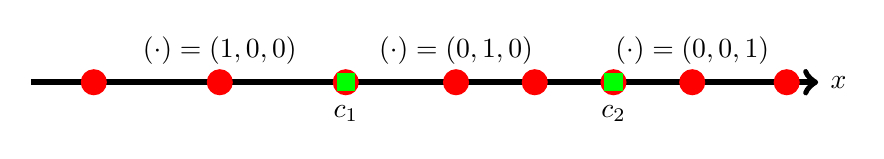
\begin{tikzpicture}[scale=0.2,every node/.style={scale=1}]
\draw[->,line width=0.08cm] (-12,0)--(38,0) node[right]{$\glssymbol{x}$};

% Original data points
\node [red,circle, fill] at (-8,0) {};
\node [red,circle, fill] at (0,0) {};
\node [red,circle, fill] at (8,0) {};
\node [red,circle, fill] at (15,0) {};
\node [red,circle, fill] at (20,0) {};
\node [red,circle, fill] at (25,0) {};
\node [red,circle, fill] at (30,0) {};
\node [red,circle, fill] at (36,0) {};


% Cut points
\node [green,rectangle,rotate=90,fill] at (8,0) {};
\node [green,rectangle,rotate=90,fill] at (25,0) {};

\node at (8,-2) {$c_1$};
\node at (25,-2) {$c_2$};

% Disc value
\node at (0,2) {$\q(\cdot) = (1,0,0)$};
\node at (15,2) {$\q(\cdot) = (0,1,0)$};
\node at (30,2) {$\q(\cdot) = (0,0,1)$};


\end{tikzpicture}
\caption{\label{fig:disc_equal_freq} Original data in \textcolor{red}{red} is discretized using an \textit{equal-freq} procedure resulting in $m=3$ intervals using the two cutpoints in \textcolor{green}{green}.}
\end{figure}



\begin{algorithm}[H]
 \KwData{$n,\glssymbol{bbx},(m_j)_1^d$}
 \KwResult{$\hat{\q}$}
 \For{$j=1$ to $d$}{
Sort $\glssymbol{bbx}^j$ by ascending order\;
Let $c_0=-\infty$, $c_{m_j} = + \infty$ and $c_{j,h} = x_{\left\lceil{{\frac{h \cdot n}{m_j}}}\right\rceil,j}$\;
Let $C_{j,h} = ]c_{j,h-1};c_{j,h}]$ and $\hat{\q}_j(\cdot) = (\hat{q}_{j,h}(\cdot))_1^{m_j}$\;
Set $\hat{q}_{j,h}(\cdot)=\mathds{1}_{C_{j,h}}(\cdot)$.
%\For{$i=1$ to $n$}{
%Set $q_i^j(x_j) = \begin{cases} 1 \text{ si } x_i^j \leq x_{\left\lceil{{\frac{n}{m_j}}}\right\rceil}^j \\ o \text{ si } x_{\left\lceil{{\frac{(o-1)*n}{m_j}}}\right\rceil}^j < x_i^j \leq x_{\left\lceil{{\frac{o*n}{m_j}}}\right\rceil}^j \\ m_j \text{ si } x_{\left\lceil{{\frac{(m_j-1)*n}{m_j}}}\right\rceil}^j < x_i^j \end{cases}$
%}
}
 \caption{\label{equal-freq-disc} \textit{equal-freq} discretization: an equal number of training observations are in each bin.}
\end{algorithm}


\subsubsection{The \textit{equal-length} algorithm} \label{app1:equal_length}

The \textit{equal-length} algorithm~\ref{equal-length-disc} is illustrated on Figure~\ref{fig:disc_equal_length}. 

\begin{figure}[!h]
\centering
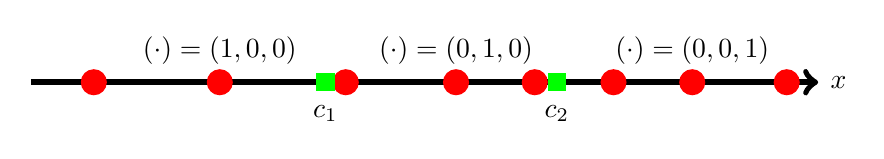
\begin{tikzpicture}[scale=0.2,every node/.style={scale=1}]
\draw[->,line width=0.08cm] (-12,0)--(38,0) node[right]{$\glssymbol{x}$};

% Original data points
\node [red,circle, fill] at (-8,0) {};
\node [red,circle, fill] at (0,0) {};
\node [red,circle, fill] at (8,0) {};
\node [red,circle, fill] at (15,0) {};
\node [red,circle, fill] at (20,0) {};
\node [red,circle, fill] at (25,0) {};
\node [red,circle, fill] at (30,0) {};
\node [red,circle, fill] at (36,0) {};


% Cut points
\node [green,rectangle,rotate=90,fill] at (6.7,0) {};
\node [green,rectangle,rotate=90,fill] at (21.4,0) {};

\node at (6.7,-2) {$c_1$};
\node at (21.4,-2) {$c_2$};

% Disc value
\node at (0,2) {$\q(\cdot) = (1,0,0)$};
\node at (15,2) {$\q(\cdot) = (0,1,0)$};
\node at (30,2) {$\q(\cdot) = (0,0,1)$};


\end{tikzpicture}
\caption{\label{fig:disc_equal_length} Original data in \textcolor{red}{red} is discretized using an \textit{equal-length} procedure resulting in $m=3$ intervals using the two cutpoints in \textcolor{green}{green}.}
\end{figure}


\begin{algorithm}[H]
 \KwData{$n,\glssymbol{bbx},(m_j)_1^d$}
 \KwResult{$\hat{\q}$}
 \For{$j=1$ to $d$}{
Let $w_j = \max{i} x_{i,j} - \min{i} x_{i,j}$\;
Let $c_0=-\infty$, $c_{m_j} = + \infty$ and $c_{j,h} = \frac{w_j \cdot h}{m_j} + \min{i} x_{i,j}$\;
Let $C_{j,h} = ]c_{j,h-1};c_{j,h}]$ and $\hat{\q}_j(\cdot) = (\hat{q}_{j,h}(\cdot))_1^{m_j}$\;
Set $\hat{q}_{j,h}(\cdot)=\mathds{1}_{C_{j,h}}(\cdot)$.
}
 \caption{\label{equal-length-disc} \textit{equal-length} discretization: each bin has the width of the training set's total support divided by the number of bins.}
\end{algorithm}



\subsection{Supervised univariate methods}

\subsubsection{The \textit{ChiMerge} algorithm}

The \textit{ChiMerge}~\cite{kerber1992chimerge} algorithm~\ref{chimerge} is a supervised (it takes into account the labels $\glssymbol{bby}$) univariate (it does not take into account the other features $\glssymbol{x}_{\{-j\}}$)). It is used indirectly in the benchmarks of Chapter~\ref{chap4} where I applied the same approach to categorical features by computing all the pairwise $\chi^2$ indepedence tests. Here we showcase a rather na\"{\i}ve implementation as a pseudo-code~\ref{chicollapse}, which in practice would perform poorly (because of exponential complexity in the number of categories $l_j$) but, from an iteration to another, a lot of $\chi^2$ tests are unaffected, so they can be stored rather than computed again. The initial and final steps of \textit{ChiMerge} are illustrated in Table~\ref{tab:chimerge_ex}. Refinements of the method, taking into account multiple testing and / or adapting $\alpha$ to each feature, were done in~\cite{liu1995chi2,wang1998concurrent,tay2002modified,su2005extended}.

%\begin{table}
%\centering
%\caption{\label{tab:chimerge_ex} p-values of $\chi^2$ tests between subsequent categories. The pair of categories the least independent (\textit{i.e.}\ with highest p-value) is $(-\infty-18,18-20)$ which should be merged into $-\infty-20$.}
%\begin{tabular}{p{2.5cm}|p{2.5cm}|p{2.5cm}|p{2.5cm}}
%Category & \# samples & \# $\{Y=1\}$ & p-value \\
%\hline
%$-\infty$-18 & 10 & 5 & \multirow{2}{*}{\textbf{1}} \\
%18-20 & 10 & 5 & \multirow{2}{*}{0.3} \\
%20-22 & 10 & 6 & \multirow{2}{*}{0.2} \\
%22-24 & 10 & 4 & \multirow{2}{*}{0.2}\\
%24-$+\infty$ & 10 & 2 & \multirow{2}{*}{0.2} \\
%\dots & \dots & \dots & \dots \\
%\end{tabular}
%\end{table}
%
%\textcolor{red}{calculer les chi 2 exacts}

\begin{table}
\caption{\label{tab:chimerge_ex} p-values of $\chi^2$ tests between subsequent categories on the iris dataset taken from~\cite{kerber1992chimerge}.}
\centering
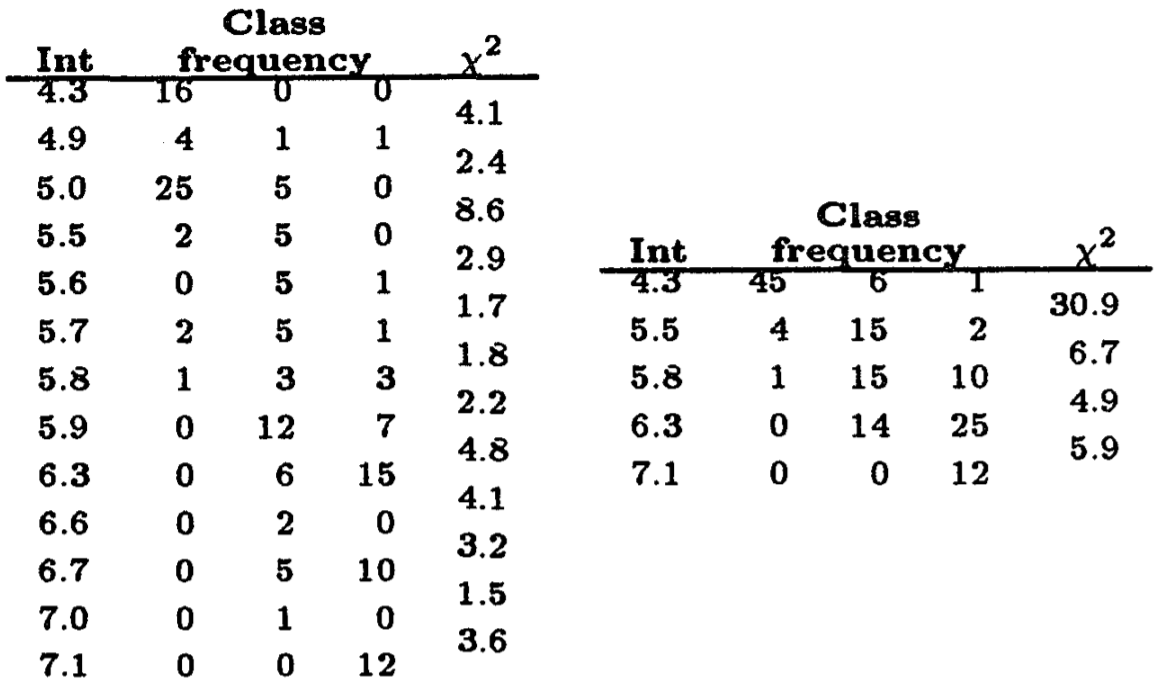
\includegraphics[width = .7\textwidth]{figures/appendix/tab_chimerge.PNG}
\end{table}

\begin{algorithm}[H]
 \KwData{$n,\glssymbol{bbx},\alpha$}
 \KwResult{$\hat{\q}$}
 \For{$j=1$ to $d$}{
 $\alpha_{\text{max}}$ = 1\;
 Sort $\glssymbol{bbx}_j$ in ascending order\;
 Let $c_0=-\infty$, $m_j = n$, $c_{m_j} = + \infty$ and $c_{j,h} = \frac{x_{i,j} + x_{i+1,j}}{2}$ for $1 \leq i \leq n-1$\;
 \While{$\alpha_{\text{max}} > \alpha$}{
Let $C_{j,h} = ]c_{j,h-1};c_{j,h}]$ and $\hat{\q}_j(\cdot) = (\hat{q}_{j,h}(\cdot))_1^{m_j}$\;
Set $\hat{q}_{j,h}(\cdot)=\mathds{1}_{C_{j,h}}(\cdot)$\;
Perform $\chi^2$ tests of independence among all contiguous pairs\:
$\chi^2_h = \sum_{h'=h}^{h+1} \sum_{y=0}^{1} \frac{ \left( \sum_{i=1}^n \mathds{1}_{y}(y_i) \hat{q}_{j,h'}(x_{i,j} ) - \frac{\sum_{i=1}^n \hat{q}_{j,h'}(x_{i,j}) \times \sum_{i=1}^n \mathds{1}_{y}(y_i)}{n} \right)^2}{\frac{\sum_{i=1}^n \hat{q}_{j,h'}(x_{i,j}) \times \sum_{i=1}^n \mathds{1}_{y}(y_i)}{n}}$ for $1 \leq h \leq m_j-1$\;
Under the null hypothesis that two consecutive intervals are independent w.r.t.\ the target $y$, $\chi^2_h$ is $\chi^2$-distributed (1 degree of freedom)\;
Let $c_{j,\argmin_h \chi^2_h} = \frac{c_{j,h} + c_{j,h+1}}{2}$ and $c_{j,h'} \leftarrow c_{j,h'+1}$ for $\argmin_h \chi^2_h < h' < m_j$\;
Let $m_j \leftarrow m_j-1$\;
Let $X \sim \chi^2$ and $\alpha_{\max} = \max_h p(X \geq \chi^2_h) = p(X \geq \min_h \chi^2_h)$.
}
}
 \caption{\label{chimerge} ChiMerge algorithm perfoming discretization by performing $\chi^2$ tests recursively at a user-defined level $\alpha$.}
\end{algorithm}


\subsubsection{The \textit{MDLP} algorithm} \label{app1:mdlp}

The \textit{MDLP} algorithm~\cite{fayyad1993multi} is an entropy-based discretization method. Contrary to ChiMerge, where at the beginning all distinct values are put into separate categories and thereafter merged (bottom-up method), MDLP recursively calculates the entropy produced by each candidate cutpoint on their subsequent binary splits.

\textcolor{red}{mettre une sorte d'arbre ici}

\begin{algorithm}[H]
 \KwData{$n,\glssymbol{bbx}$}
 \KwResult{$\hat{\q}$}
 \For{$j=1$ to $d$}{
}
 \caption{\label{mdlp} MDLP algorithm recursively perform discretization with an information gain criterion.}
\end{algorithm}


\subsection{Proposal: \textit{glmdisc}}


\subsubsection{\textit{glmdisc} with neural networks}

This section describes the \textit{glmdisc}-NN algorithm developed in Chapter~\ref{chap4} and examplifies it on simulated data in Figure~\ref{fig:animNN}

\begin{algorithm}[H]
 \KwData{$(\bm{x},\bm{y})$}
 \KwResult{$\bm{e},(\beta_k)_1^{d_1}$,(T$^k)_{d_1}^{d_1+d_2}$}
 \caption{\label{NN-disc} \textit{glmdisc}-NN: supervised multivariate discretization for logistic regression with neural networks.}
\end{algorithm}

%\begin{figure}[!h]
%\begin{animateinline}[poster=first, controls=all, palindrome, autopause, autoresume, width=\textwidth, height=7cm]{3}
%\multiframe{200}{i=1+1}{\input{R_CODE_FIGURES/appendix/animation_disc_tensorflow/False_simulated_data/feature_0_iteration_\i.tex}}%
%\end{animateinline}
%\caption{\label{fig:animNN} bla.}
%\end{figure}


\textcolor{red}{à décommenter // ajouter caption}

\subsubsection{\textit{glmdisc} with an \gls{sem} algorithm}

This section describes the \textit{glmdisc}-SEM algorithm developed in Chapter~\ref{chap4} and examplifies it on simulated data in Figure~\ref{fig:animSEM}

\begin{algorithm}[H]
 \KwData{$((\glssymbol{bbx}_j)_1^{d_1} \text{ (continuous features)},(\glssymbol{bbx}_j)_{d_1}^{d_1 + d_2} \text{ (categorical features)}, \glssymbol{bby}),\max\_\text{iter},\bm{m}_\text{start}$}
 \KwResult{$\hat{\q}$}
 Initialization of $\bm{q}^{(0)}$ at random\;
 $r = 0$\;
 \While{$r < \max\_\text{iter}$}{
  Adjust logistic regression $\hat{\gamma}^{(r)} = \argmax_\gamma \ell(\gamma;\q^{(r)}, \bm{y})$\;
  ${\q^{(r+1)}} \leftarrow {\q^{(r)}}$\;
  \For{$k \leftarrow 1$ \KwTo $d_1$}{
   Adjust multinomial logistic regression $\hat{\beta}_k^{(r)} = \argmax_\beta \ell(\beta;\glssymbol{bbx}_k,\q_k^{(r)})$\;
   ${\q_k^{(r+1)}} \leftarrow$ Mult$(p_{\hat{\gamma}^{(r)}}(\bm{y}|\q^{(r+1)}) p_{\hat{\beta}^{k(r)}}(\q_{k} | \glssymbol{bx}_k))$\;
   ${\q_k^{\text{MAP}(r+1)}} \leftarrow \argmax_j p_{\hat{\beta}^{k(r)}}(\bm{E}^{k}=j | \bm{x}^k))$\;
   }
  \For{$k \leftarrow d_1+1$ \KwTo $d_1+d_2$}{
   Form the contingency table T$_k^{(r)}$ of $\q_k^{(r)}$ against $\glssymbol{bbx}_k$, calculate the frequencies of each value of $({q}_{k},x_k)$\;
	${\q_k^{(r+1)}} \leftarrow$ Mult$(p_{\hat{\gamma}^{(r)}}(\bm{y}|\q^{(r+1)}) p_{T_k^{(r)}}(\q_{k} | \glssymbol{bx}^k))$\;
	${\q_k^{MAP(r+1)}} \leftarrow \argmax_j p_{T_k^{(r)}}(\q_{k}=j | \glssymbol{bx}_k))$\;
	}
   $r \leftarrow r+1$\;
 }
 Choose the best quantization and logistic regression model from $ $ where $(p_{\hat{\eta}^{(r)}}(\bm{y} | \bm{e}_{MAP}^{(r)}))_1^{Max}$.
 \caption{\label{SEM-disc} \textit{glmdisc}-SEM: supervised multivariate discretization for logistic regression with an \gls{sem} algorithm.}
\end{algorithm}

%\begin{figure}[!h]
%\begin{animateinline}[poster=first, controls=all, palindrome, autopause, autoresume, width=\textwidth, height=7cm]{5}
%\multiframe{200}{i=1+1}{\input{R_CODE_FIGURES/appendix/animation_disc_SEM/sem_simulated_data/sem_feature_1_iter_\i.tex}}%
%\end{animateinline}
%\caption{\label{fig:animSEM} bla.}
%\end{figure}

\textcolor{red}{à décommenter // ajouter caption  et numéro itération}


\section{Factor levels grouping method} \label{app1:chicollapse}

As part of Chapter~\ref{chap4}, I gave results for competing methods MDLP / $\chi^2$ tests where the $\chi^2$ tests can be explicited in Algorithm~\ref{chicollapse} which I called ChiCollapse. My rather na{\"\i}ve implementation (where, as in the pseudo-code~\ref{chicollapse}, all pairwise $\chi^2$ tests are recalculated at each step) is available as a gist on Github at \url{https://gist.github.com/adimajo/eb007492007d650091f6bd7cb2047493}. An example of the resulting usage of the grouped levels in a predictive setting is also given as a gist on Github at \url{https://gist.github.com/adimajo/8f8401b59ba838c65534673842b0f60d}.

\begin{algorithm}[H]
 \KwData{$n,\glssymbol{bbx},\alpha$}
 \KwResult{$\hat{\q}$}
 \For{$j=1$ to $d$}{
 $\alpha_{\text{max}}$ = 1\;
 Let $C_{j,h} = \{h\}$ for $1 \leq i \leq l_j$\;
 \While{$\alpha_{\text{max}} > \alpha$}{
Let $\hat{\q}_j(\cdot) = (\hat{q}_{j,h}(\cdot))_1^{m_j}$\;
Set $\hat{q}_{j,h}(\cdot)=\mathds{1}_{C_{j,h}}(\cdot)$\;
Perform all pairwise $\chi^2$ tests of independence among all contiguous pairs\:
$\chi^2_{h_1,h_2} = \sum_{h'=h_1}^{h_2} \sum_{y=0}^{1} \frac{ \left( \sum_{i=1}^n \mathds{1}_{y}(y_i) \hat{q}_{j,h'}(x_{i,j} ) - \frac{\sum_{i=1}^n \hat{q}_{j,h'}(x_{i,j}) \times \sum_{i=1}^n \mathds{1}_{y}(y_i)}{n} \right)^2}{\frac{\sum_{i=1}^n \hat{q}_{j,h'}(x_{i,j}) \times \sum_{i=1}^n \mathds{1}_{y}(y_i)}{n}}$ for $1 \leq h_1 < h_2 \leq m_j$\;
Under the null hypothesis that two factor levels are independent w.r.t.\ the target $y$, $\chi^2_{h_1,h_2}$ is $\chi^2$-distributed (1 degree of freedom)\;
Let $(h_1,h_2) = \argmin_{h_1,h_2} \chi^2_{h_1,h_2}$, $C_{j,h_1} = C_{j,h_1} \cup C_{j,h_2}$ and $C_{j,h} \leftarrow C_{j,h+1}$ for $h_2 \leq h \leq m_j$\;
Let $m_j \leftarrow m_j-1$\;
Let $X \sim \chi^2$ and $\alpha_{\max} = \max_{h_1,h_2} p(X \geq \chi^2_{h_1,h_2}) = p(X \geq \min_{h_1,h_2} \chi^2_{h_1,h_2})$.
}
}
 \caption{\label{chicollapse} ChiCollapse algorithm: adaptation of ChiMerge to categorical features.}
\end{algorithm}


\section{Interaction discovery methods}



\section{Logistic regression-based trees}


\subsection{\Gls{lmt}}


\subsection{\Gls{mob}}




\printbibliography[heading=subbibliography, title=References of Appendix A]